\subsection{Inter-Intergrated Circuit (I2C)} \label{grund-i2c-subsubsec}

\todo[inline]{Verantwortlich: Kevin, Jonas}

Das Inter-Integrated Circuit (kurz: I2C, gesprochen I-Quadrat-C), oder auch Inter IC-Bus, ist wie das in Kapitel 2.1. besprochene SPI ein synchrones und serielles Bussystem. Dieses wurde 1982  von Philips entwickelt und ermöglicht eine Kommunikation zwischen verschiedenen integrierten Schaltungen (ICs, engl. Integrated Circuit) für die nur zwei Leitungen benötigt werden. Das Protokoll erlaubt es bei einer Adressierung von sieben Bit, mit bis zu 128 Slaves zu kommunizieren. Vorteil dieses Bussystems ist die Kommunikation mit einem oder mehreren Master ICs. Ein I2C-Bus mit mehreren Master ICs wird als "Multi-Master-Bus"bezeichnet. Die Übertragungsraten bei Mikrocontrollern betragen bis zu 400 kbit/s und können in leistungsstärkeren Systemen bis zu 3,4 MBit/s erreichen. Taktgeschwindigkeiten sollten sich aber immer am langsamsten IC im Bus orientieren, damit es nicht zu kommunikationsproblemen kommt. Slaves sind mit einer eigenen, individuellen fest zugeordneten Adresse codiert. Über einen Broadcastkanal können analog alle Slaves in einem Verbund gleichzeitig angesprochen werden. Die Adressierung erfolgt dabei stehts durch den Master. Das heißt, dass Slaves niemals selbständig eine Kommunikation starten können. Lediglich der Master teilt nach Versenden der Slave-Adresse mit (Adresse ist dabei sieben Bit lang), ob er im Folgenden Daten senden oder von dem jeweiligen Gerät empfangen möchte (das 8. Bit), die dann entweder vom Master oder vom Slave auf den Bus gelegt werden. Also initiert der Master den Datentransfer und synchronisiert den Takt, mit dem der Transfer abläuft. Nach erfolgreicher Kommunikation gibt der Master den Bus anschließend wieder frei. Betrachtet man die Kommunikation auf Bitebene, werden durch eine Kombination der Zustände von Takt- und Datenleitung die Start-/Stopp-Bedingungen durch den Master eingeleitet. Um die erfolgreiche Kommunikation zwischen Master und Slave sicherzustellen, wird für die Quittierung zwischen einzelnen Datenpaketen und nach Übertragung der gesamten Daten ein Acknowledge bzw. Not-Acknowledge versendet.

\begin{figure}[H] \centering
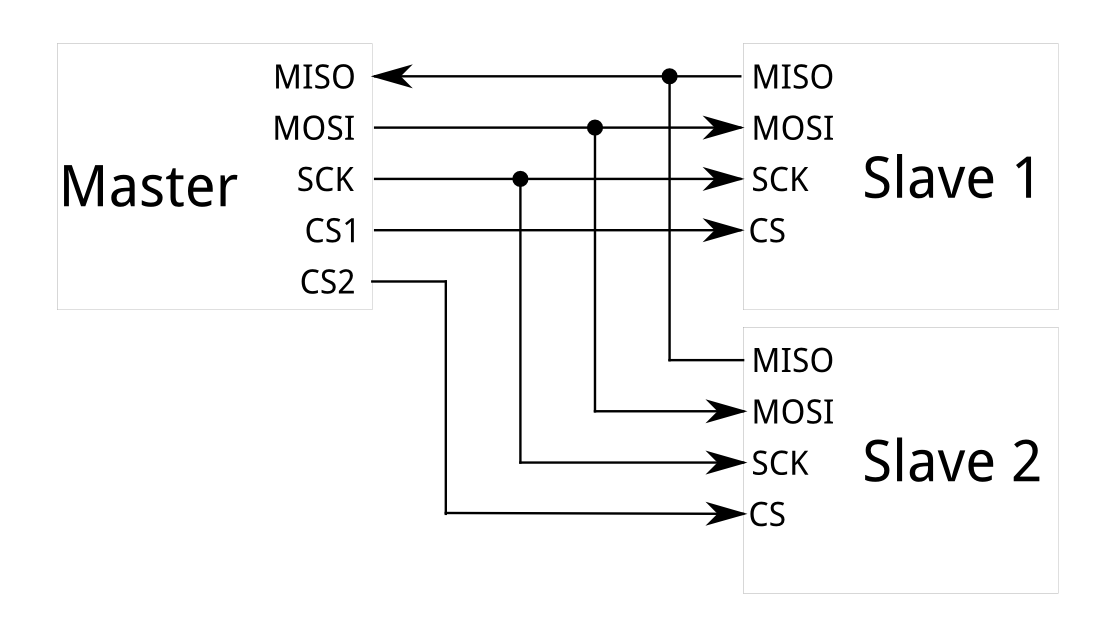
\includegraphics[width=\textwidth]{Images/I2C_multiple_slaves.png} 
\vspace{-0.3cm} 
\caption{ I2C-Master mit 2 Slaves.}
\label{fig-elise} 
\end{figure}